\documentclass[10pt]{beamer}

% mac版,texShop 中Typeset选择 XeLaTex 

%%%%%%%%%%%%%%%%%%%%%%%%%%%%%%%%%%%%%
\usepackage[slantfont,boldfont]{xeCJK}
%\input{xecjkfonts},CJKtextspaces
\setCJKmainfont{STKaiti}   % STFangsong 设置缺省中文字体
\setCJKmonofont{SimSun}   % 设置等宽字体
\setmainfont{Times} % 英文衬线字体
\setmonofont{Times} % 英文等宽字体
\setsansfont{Times} % 英文无衬线字体
%%%%%%%%%%%%%%%%%%%%%%%%%%%%%%%%%%%%%%

\mode<presentation> {
  %\usetheme{Madrid}
  %\usetheme{Singapore}
  \usetheme{Warsaw}
  \setbeamercovered{transparent}
 % \usefonttheme[onlymath]{serif}  
 \usefonttheme{professionalfonts}%{structurebold}
 % \usefonttheme[onlymath]{structurebold}
  \usecolortheme{rose}
}

\usepackage[english]{babel}
%\usepackage[latin1]{inputenc}

%\usepackage{times}
%\usepackage[T1]{fontenc}


%\usepackage{epsfig}
\usepackage{graphics}
\usepackage{color}
\usepackage{amsmath,amssymb,mathrsfs}
\usepackage{amsfonts,stmaryrd}
%\usepackage{thmmarks}
%\usepackage{}



\newcommand\frakfamily{\usefont{U}{yfrak}{m}{n}}
\DeclareTextFontCommand{\textfrak}{\frakfamily}
\def\diag{\mathrm{diag}}


\title[数值计算方法]{数值计算方法}
\subtitle{-数值微积分}


\subject{Talks}

% If you have a file called "university-logo-filename.xxx", where xxx
% is a graphic format that can be processed by latex or pdflatex,
% resp., then you can add a logo as follows:

% \pgfdeclareimage[height=0.5cm]{university-logo}{university-logo-filename}
% \logo{\pgfuseimage{university-logo}}

%\pgfdeclareimage[height=0.5cm]{university-logo}{ncsu_logo}
%\logo{\pgfuseimage{university-logo}}

% Delete this, if you do not want the table of contents to pop up at
% the beginning of each subsection:
%\AtBeginSubsection[] {
%  \begin{frame}<beamer>
%    \frametitle{Outline}
%    \tableofcontents[currentsection,currentsubsection]
%  \end{frame}
%}

% If you wish to uncover everything in a step-wise fashion, uncomment
% the following command:

% \beamerdefaultoverlayspecification{<+->}


\setbeamertemplate{theorems}[numbered]
\setbeamertemplate{caption}[numbered]


\newtheorem{proposition}[theorem]{Proposition}

%%%%%%%%%%%%%%%%%%%%%%%%%%%
% REMARK-STYLE-ENVIRONMENTS %
%%%%%%%%%%%%%%%%%%%%%%%%%%%
\newcounter{remark}
% \numberwithin{theorem}{section}
\def\openrem#1#2{\refstepcounter{remark}\bigskip

{\noindent\bf#1~\theremark\if#2!{. }\else{ (#2).}\fi}
\it}
\def\thmskip{}
\newenvironment{remark}[1][!]{\openrem{Remark}{#1}}{\thmskip}

%%%%%%%%%%%%%%%%%%%%%%%%%%%%
%% AlGORITHM-STYLE-ENVIRONMENTS %
%%%%%%%%%%%%%%%%%%%%%%%%%%%%
\newcounter{algorithm}
% \numberwithin{theorem}{section}
\def\openalg#1#2{\refstepcounter{algorithm}\bigskip

{\noindent\bf#1~\thealgorithm\if#2!{. }\else{ (#2).}\fi}
\it}
\def\thmskip{}
\newenvironment{algorithm}[1][!]{\openrem{Algorithm}{#1}}{\thmskip}
%
%
%%%%%%%%%%%%%%%%%%%%%%%%%%%%
%% Result-STYLE-ENVIRONMENTS %
%%%%%%%%%%%%%%%%%%%%%%%%%%%%
%\newcounter{result}
%\def\openrem#1#2{\refstepcounter{result}\bigskip
%{\noindent \it \bfseries#1~\theremark\if#2!{. }\else{ (#2). }\fi}}
%\newenvironment{result}[1][!]{\openrem{Result}{#1}}{\qed}




%%%%%%%%%%%%%%%%%%%%%%%%%%%
%Redefine the Symbols%
%%%%%%%%%%%%%%%%%%%%%%%%%%%

\def\mathbi#1{\textbf{\em #1}}

% integrals
\def\dx{\,{\rm d}x}
\def\dxb{\,{\rm d}\boldsymbol{x}}
\def\dy{\,{\rm d}y}
\def\dt{\,{\rm d}t}
\def\ds{\,{\rm d}s}
\def\du{\,{\rm d}u}

\def\dr{\,{\rm d}r}
\def\dtheta{\,{\rm d}\theta}

\def\dd{{\rm d}}

\def\intOm{\int_{\Omega}}
\def\intbOm{\int_{\partial \Omega}}

% differences
\def\Dx{\Delta x}
\def\Dt{\Delta t}
\def\D{\Delta}


% operators
\def\Ls{\mathscr{L}}

% matirices
\def\Js{\mathscr{J}}


%fields%
\def\R{\mathbb{R}}
\def\N{\mathbb{N}}
\def\Z{\mathbb{Z}}

%Spaces%
\def\H{\mathbb{H}}
\def\L{\mathbb{L}}
\def\P{\mathbb{P}}


\def\U{\mathbb{U}}
\def\V{\mathbb{V}}
\def\W{\mathbb{W}}
\def\X{\mathbb{X}}
\def\Y{\mathbb{Y}}

\def\Cinfty{C^\infty}




%vectors%
\def\ab{\boldsymbol{a}}
\def\bb{\boldsymbol{b}}
\def\cb{\boldsymbol{c}}
\def\db{\boldsymbol{d}}
\def\eb{\boldsymbol{e}}
\def\fb{\boldsymbol{f}}
\def\gb{\boldsymbol{g}}
\def\hb{\boldsymbol{h}}
\def\nb{\boldsymbol{n}}
\def\rb{\boldsymbol{r}}
\def\sb{\boldsymbol{s}}


\def\ub{\boldsymbol{u}}
\def\vb{\boldsymbol{v}}
\def\wb{\boldsymbol{w}}
\def\xb{\boldsymbol{x}}
\def\yb{\boldsymbol{y}}
\def\zb{\boldsymbol{z}}

\def\Bb{\boldsymbol{B}}
\def\Cb{\boldsymbol{C}}
\def\Eb{\boldsymbol{E}}
\def\Fb{\boldsymbol{F}}
\def\Ib{\boldsymbol{I}}
\def\Kb{\boldsymbol{K}}
\def\Ob{\boldsymbol{O}}
\def\Qb{\boldsymbol{Q}}
\def\Rb{\boldsymbol{R}}
\def\Sb{\boldsymbol{S}}
\def\Ub{\boldsymbol{U}}
\def\Vb{\boldsymbol{V}}
\def\Wb{\boldsymbol{W}}
\def\Xb{\boldsymbol{X}}
\def\Yb{\boldsymbol{Y}}
\def\Zb{\boldsymbol{Z}}

%domains%
\def\Om{\Omega}
\def\bd{\partial}
\def\bOm{\bar{\Omega}}

%bold symbols%
\def\alphab{\boldsymbol{\alpha}}
\def\phib{\boldsymbol{\varphi}}

%energy%
\def\Jc{\mathcal{J}}
\def\Oc{\mathcal{O}}

%Greeks%
\def\vphi{\varphi}

%Special Functions%
\def\supp{\rm{supp}}
\def\sym{\rm{sym}}

\def\gradu{\nabla u}
\def\gradv{\nabla v}

%Mesh%
\def\Ts{\mathcal{T}}

\def\mach{\rm{mach}}


\begin{document}

\setbeamertemplate{itemize item}[triangle]

\begin{frame}
\titlepage
\end{frame}


\begin{frame}
  \frametitle{本节概要}
  \tableofcontents%[pausesections]
  % You might wish to add the option [pausesections]
%  \begin{itemize}
%  \item 显示Euler法及其误差分析
%  \item Taylor展开法
%  \item 
%  \end{itemize}
\end{frame}


\section{数值微分}

\begin{frame}
\frametitle{数值微分}
如果一个函数是基本函数(如$f(x) = \sin x$或基本函数通过复合构成的(如$f(x) = \sin^3 ( x^{\tan x} \cosh x)$),那么这个函数的导数可以利用求导法则求出。

\vspace{0.2cm}

如果一个函数是由测量或者计算结果直接生成的因而只有离散点上的值,那么这个函数的求导就不能够用求导法则来得到,因而需要数值微分对这个函数的导数进行近似。
\end{frame}


\subsection{数值微分公式}

\begin{frame}
\frametitle{两点向前差分}
\begin{definition}[微分]
如果以下的极限存在,则一个函数在$x$点上的导数$f'(x)$是指
\begin{equation}
f'(x) = \lim_{h \rightarrow 0} \frac{f(x+h) - f(x)}{h}.
\end{equation}
\end{definition}
这个公式给了我们对导数的一个最基本的近似。因为计算机所能表示的数不能够无穷小,我们用差分代替微分,取一个比较小的$h>0$,我们就得到了$f'(x)$的近似
\begin{equation}
\label{eq: foward difference}
f'(x) \approx \frac{f(x+h) - f(x)}{h},
\end{equation}
这个公式称为两点向前差分公式。
\end{frame}


\begin{frame}
\frametitle{两点向前差分公式的误差}
两点差分公式的精确程度是多少呢?我们可以由Taylor展式得到。根据Taylor展式,我们有
\begin{equation}
f'(x) = \frac{f(x+h)-f(x)}{h} - \frac{h}{2} f''(\xi),
\end{equation}
其中$\xi \in [x, x+h]$。根据这个公式通过移项我们得到
\begin{equation}
|f'(x) - \frac{f(x+h) - f(x)}{h}|=  | \frac{h}{2}f''(\xi)|.
\end{equation}
我们发现通过两点差分公式\eqref{eq: foward difference}得到的对$f'(x)$的近似与$f'(x)$的误差在$f''(x)$附近有界的时候近似的与$h$成正比。我们称两点差分公式是一个$O(h)$的方法。一般的,如果某个方法的误差是$O(h^n)$的,我们称这个方法是$n$阶的。理论上说,当$h \rightarrow 0$时,两点差分公式的误差趋于$0$。当然,由于计算机只具有有限精度,所以$h$只能是一个比较小的数而不能无限趋近于$0$。
\end{frame}


\begin{frame}
\frametitle{两点向前差分公式的举例}
\begin{example}
利用两点差分公式,取$h = 0.1$来计算$f(x) = \frac{1}{x}$在$x = 2$的导数。
\end{example}
利用两点差分公式
\begin{equation}
f'(x) \approx \frac{f(x + h) - f(x)}{h} = \frac{\frac{1}{2.1} - \frac{1}{2}}{0.1} \approx -0.2381.
\end{equation}
将这个近似与$f'(x) = -\frac{1}{x^2}$在$x = 2$的值作比较,得到(真实的)误差为
\begin{equation}
-0.2391 - (-0.2500) = 0.0119.
\end{equation}
根据误差公式,$\frac{h}{2}f''(\xi)$在$\xi \in [2, 2.1]$时在
\begin{equation*}
(0.1) f''(2) = 0.1 \times 2\frac{1}{2^3} = 0.0125 \text{ \quad 与 \quad} (0.1) f''(2.1) \approx 0.0108
\end{equation*}
之间。可以看到误差满足这个估计。
\end{frame}


\begin{frame}
\frametitle{中心差分公式}
我们可以利用Taylor展式寻找更高阶的数值微分公式。令$h >0$且$f(x)$三阶连续可导,则
\begin{align}
f(x+h) = f(x) + hf'(x) + \frac{h^2}{2} f''(x) + \frac{h^3}{6} f'''(\xi_1) \nonumber \\
f(x-h) = f(x) - hf'(x) + \frac{h^2}{2} f''(x) - \frac{h^3}{6} f'''(\xi_2)
\end{align}
其中$\xi_1 \in [x, x+h]$,$\xi_2 \in [x-h,x]$。以上两式相加得到
\begin{equation}
f'(x) = \frac{f(x+h) - f(x-h)}{2h} - \frac{h^2}{12} f'''(\xi_1) - \frac{h^2}{12} f'''(\xi_2).
\end{equation}
上式右端第一项就是中心差分公式。可以观察到,中心差分公式是一个$O(h^2)$的公式。
\end{frame}


\begin{frame}
\frametitle{中心差分公式的误差}
为了得到中心差分公式的更为简洁的误差表达式,我们首先有以下定理
\begin{theorem}[中值定理的一般形式]
令$f(x)$是$[a,b]$上的连续函数,$x_1, \ldots, x_n$是$[a,b]$上的点,$a_1, \ldots, a_n >0$。存在$\xi \in [a,b]$使得
\begin{equation}
(a_1 + \ldots + a_n) f(\xi) = a_1 f(x_1) + \ldots a_n f(x_n).
\end{equation}
\end{theorem}
根据这个定理,令$a_1 = \frac{1}{2}$,$a_2 = \frac{1}{2}$,则存在$\xi \in [x - h, x+h]$使得
\begin{equation}
f'(x) = \frac{f(x+h) - f(x-h)}{2h} - \frac{h^2}{6} f'''(\xi).
\end{equation}
\end{frame}


\begin{frame}
\frametitle{中心差分公式举例}
\begin{example}
利用中心差分公式,取$h = 0.1$,计算$f(x) = \frac{1}{x}$在$x = 2$处的导数的近似值。
\end{example}
利用中心差分公式
\begin{equation}
f'(x) \approx \frac{f(x+h) - f(x-h)}{2h} = \frac{\frac{1}{2.1} - \frac{1}{1.9}}{0.2} \approx -0.2506.
\end{equation}
与$f'(2)$相比,误差为$0.0006$,可以看作向前差分的改进。
\end{frame}


\begin{frame}
\frametitle{高阶导数近似}
利用函数$f(x)$的Taylor展式,可以得到对$f(x)$的高阶导数的近似,例如
\begin{equation}
f(x+h) + f(x-h) - 2f(x) = h^2 f''(x) + \frac{h^4}{24} f^{(4)}(\xi_1) + \frac{h^4}{24} f^{(4)}(\xi_2),
\end{equation}
从而
\begin{equation}
f''(x) = \frac{f(x-h) - 2f(x) + f(x+h)}{h^2} - \frac{h^2}{12} f^{(4)}(\xi),
\end{equation}
其中$\xi, \xi_1, \xi_2 \in [x-h, x+h]$.
\end{frame}


\subsection{舍入误差}

\begin{frame}
\frametitle{舍入误差}
数值微分事实上是一个不稳定的过程。我们可以发现,当$h \rightarrow 0$时,$f(x)$与$f(x+h)$是非常接近的,也就是说在计算数值微分的时候,我们需要对两个非常相近的数字进行相减,进而会丢失大量的有效数字,而且这个问题无法避免。我们用以下例子来展示这个问题。
\begin{example}
计算$f(x) = e^x$在$x = 0$处的导数的近似。
\end{example}

利用向前差分公式
\begin{equation}
\label{eq: foward difference exp(x)}
f'(x) \approx \frac{e^{x +h} - e^{x}}{h}.
\end{equation}
利用中心差分公式
\begin{equation}
\label{eq: centered difference exp(x)}
f'(x) \approx \frac{e^{x +h} - e^{x-h}}{2h}.
\end{equation}
计算结果如下表。
\end{frame}


\begin{frame}
\frametitle{舍入误差}
\begin{figure}
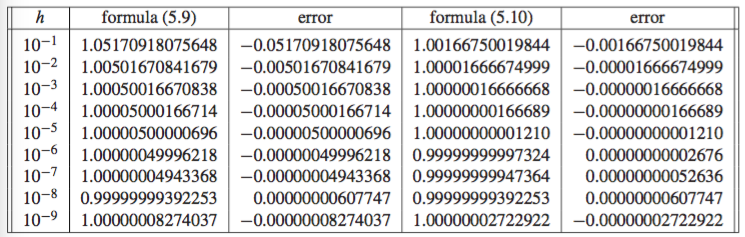
\includegraphics[width=10cm]{figs/5-1_Rounding_Error-1} 
%\caption{点$(0,1),(2,2),(3,4)$被$P(x) = \frac{1}{2}x^2 - \frac{1}{2}x+ 1$插值} 
\end{figure}
可以看到,无论哪种方法误差达到一定的值之后都会有一个上升,而不是随着$h$的减小一直递减。

\vspace{0.2cm}

这种现象实际上给我们在编程实践中一个方便,这就是在我们需要编写某个函数的导数时,可以将我们编写的导数与有限差分所求得的导数进行相减,如果误差满足这样一种先递减再递增的趋势,我们就可以确认我们编写的导数是正确的。如果不是这样一个趋势,比如误差保持在一定的水平,那么我们编写的导数肯定是有问题的。
\end{frame}


\begin{frame}
\frametitle{舍入误差分析}
我们对舍入误差进行进一步的详细分析,尝试寻找使得误差最小的$h$。由于浮点数是有限精度的,我们可以令$f(x+h)$的浮点表示为$\hat{f}(x+h)$,$f(x-h)$的浮点表示为$\hat{f}(x-h)$,满足
\begin{align}
\hat{f}(x+h) &= f(x+h) + \epsilon_1, \nonumber \\
\hat{f}(x-h) &= f(x-h) + \epsilon_2.
\end{align}
利用中心差分公式,我们得到
\begin{figure}
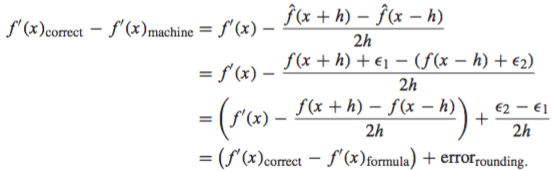
\includegraphics[width=9cm]{figs/5-1_Rounding_Error-2} 
%\caption{点$(0,1),(2,2),(3,4)$被$P(x) = \frac{1}{2}x^2 - \frac{1}{2}x+ 1$插值} 
\end{figure}
\end{frame}


\begin{frame}
\frametitle{舍入误差分析}
由上面的式子,我们得到
\begin{align}
 |f'(x)_{\rm{correct}} - f'(x)_{\rm{machine}}|  \le \frac{h^2}{6}f'''(\xi) + \frac{\epsilon_{\rm{mach}}}{h} := E(h).
\end{align}
我们利用求$E'(h)=0$的点寻找$E(h)$的极小值点,得到
\begin{align}
0 = E'(h) &= -\frac{\epsilon_{\rm{mach}}}{h^2} + \frac{f'''(\xi)}{3}h \nonumber \\
           h & = (\frac{3\epsilon_{\rm{mach}}}{f'''(\xi)})^{\frac{1}{3}}.
\end{align}
在双精度表示中,$\epsilon_{\rm{mach}}^{\frac{1}{3}} \approx 10^{-5}$,与之前表格中的情况是一致的。
\end{frame}



\subsection{外推}

\begin{frame}
\frametitle{外推}
由于舍入误差的原因,微分公式的精度是有限的,如果需要进一步提高精度我们应该如何做呢?这里我们介绍一种提高精度的有效方法,这就是外推法。

\vspace{0.2cm}

假设我们要求的一个量$Q$满足
\begin{equation}
Q \approx F(h) + K h^n ,
\end{equation}
其中$K$是一个近似的常数,则我们可以利用
\begin{equation}
\label{eq: extrapolation 1}
Q \approx \frac{2^n F(\frac{h}{2}) - F(h)}{2^n - 1}
\end{equation}
来得到$Q$得更高阶近似。这种方法叫作外推
\end{frame}


\begin{frame}
\frametitle{外推法的推导}
我们假设$Q$的$n$阶近似为$F_n(h)$,满足
\begin{equation}
Q = F_n(h) + Kh^n + O(h^{n+1}),
\end{equation}
则
\begin{equation}
Q = F_n(\frac{h}{2}) + K\frac{h^n}{2^n} + O(h^{n+1}).
\end{equation}
利用\eqref{eq: extrapolation 1}得到
\begin{figure}
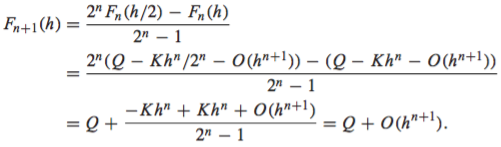
\includegraphics[width=9cm]{figs/5-1-3_Extrapolation-1} 
%\caption{点$(0,1),(2,2),(3,4)$被$P(x) = \frac{1}{2}x^2 - \frac{1}{2}x+ 1$插值} 
\end{figure}
从而$F_{n+1}(h)$是一个对$Q$的$n+1$阶近似。
\end{frame}


\begin{frame}
\frametitle{外推法举例}
\begin{example}
利用中心差分公式的外推法得到$f'(x)$精度为$3$阶的差分公式。
\end{example}
我们令
\begin{equation}
F_2(h) = \frac{f(x+h) - f(x-h)}{2h}
\end{equation}
为$2$阶的差分公式,则根据外推公式
\begin{figure}
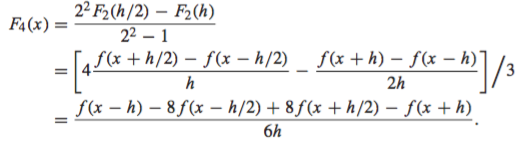
\includegraphics[width=9cm]{figs/5-1-3_Extrapolation-2} 
%\caption{点$(0,1),(2,2),(3,4)$被$P(x) = \frac{1}{2}x^2 - \frac{1}{2}x+ 1$插值} 
\end{figure}
\end{frame}

\begin{frame}
\frametitle{外推法举例}
这里有几点值得注意:
\begin{enumerate}
\item 通过外推得到的公式本来应该是$F_3(h)$,但是由于一些误差项出现了抵消,因此实际上通过分析可以知道外推得到的公式是$4$阶的,即$F_4(h)$。
\item 我们通过外推法得到了新的计算一阶导数的公式,但是这个公式我们并不直接使用,而是仍然利用外推公式来进行计算。这是一方面是因为新的公式不一定都能像上面的公式一样容易的得到;另一方面新的公式有可能因为含有更多的几乎相等的数相减而增加舍入误差。
\end{enumerate}
\end{frame}

%%%%%%%%%%%%%%%%%%%%%%%%%%%%%%%%%%%%%%%%%%



\section{数值积分}


\begin{frame}
\frametitle{数值积分}
微积分的另一大问题就是积分。虽然我们尝试过种类繁多的函数的积分,也有换元积分法和分部积分法两种积分方法,但事实上,绝大部分的函数是没有显示的原函数的,也就是说,绝大部分的函数不能够通过积分方法找到由基本函数(加减乘除、多项式、$\sin$、$\cos$等)通过复合得到的函数。例如
\begin{equation}
f(x) = \cos x^2,
\end{equation}
就没有能够通过初等函数表示的原函数。

\vspace{0.2cm}

实际应用中,求函数的原函数,即求不定积分并不一定是我们需要,尤其是对于定积分来说,我们实际上只需要求函数在某个区间上的积分的值,而利用不定积分得到这个积分的值只是根据Newton-Liebniz定理找到的一个“简便”的途径而已。

\vspace{0.2cm}

因此,我们可以换一种思路,利用数值的方法来求一个函数在某个区间上的定积分。这个过程就叫作数值积分。
\end{frame}


\subsection{Newton-Cotes积分公式}

\begin{frame}
\frametitle{Newton-Cotes积分公式}
我们利用上一讲的结论来寻找积分公式。无法求积分的根本在于被积函数$f(x)$的原函数无法找到,那么一个基本的想法就是用一个可以找到原函数的函数$P(x)$去逼近$f(x)$,通过对$P(x)$进行精确积分来近似$f(x)$的积分。

\vspace{0.2cm}

如果我们用多项式$P(x)$对$f(x)$进行插值,那么$P(x)$就是$f(x)$的一个逼近。利用多项式$P(x)$的精确积分来近似$f(x)$的积分的方法就称为Newton-Cotes数值积分公式。
\end{frame}


\begin{frame}
\frametitle{Newton-Cotes积分公式}
为了后面讨论的方便,我们首先给出三个特别的多项式的积分精确值。

\vspace{0.2cm}

第一个是经过$(0,0)$和$(h,1)$点的线性函数在$[0,h]$上的积分为
\begin{equation}
\int_0^h \frac{x}{h} \dx = \frac{h}{2}.
\end{equation}
第二个是经过点$(-h,0)$,$(0,1)$,$(h,0)$的抛物线$P(x)$在$[-h, h]$上的积分
\begin{equation}
\label{eq: integral parabola 1}
\int_{-h}^h P(x) \dx = x - \frac{x^3}{3h^2} = \frac{4}{3}h.
\end{equation}
第三个是经过点$(-h,1)$,$(0,0)$,$(h,0)$的抛物线$P(x)$在$[-h, h]$上的积分
\begin{equation}
\label{eq: integral parabola 2}
\int_{-h}^h P(x) \dx  = \frac{1}{3}h.
\end{equation}
\end{frame}


\begin{frame}
\frametitle{Newton-Cotes积分公式}
三个积分如下图
\begin{figure}
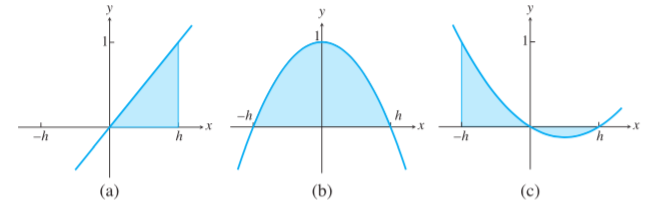
\includegraphics[width=11cm]{figs/5-2-1_Newton-Cotes-1} 
%\caption{$f(x) = x^3 + x -1$的图像} 
\end{figure}
\end{frame}


\begin{frame}
\frametitle{梯形公式}
我们首先考虑最简单的情况,用一次多项式对原函数进行插值后对插值函数进行积分。假设积分区域为$[x_0, x_1]$,函数$f(x)$在$x_0, x_1$上的值为$y_0 = f(x_0)$,$y_1 = f(x_1)$。则对原函数进行线性插值得到
\begin{equation*}
f(x) = y_0 \frac{x - x_1}{x_0 - x_1} + y_1 \frac{x - x_0}{x_1 - x_0} + \frac{(x - x_0)(x - x_1)}{2!}f''(c_x) = P(x) + E(x), 
\end{equation*}
其中$c_x=c(x)$可以证明是关于$x$的连续函数。对上式两边同时积分得到
\begin{equation}
\label{eq: trapezoid rule original}
\int_{x_0}^{x_1} f(x) \dx = \int_{x_0}^{x_1} P(x) \dx + \int_{x_0}^{x_1} E(x) \dx.
\end{equation}
\end{frame}


\begin{frame}
\frametitle{梯形公式}
对上式右端第一项进行积分得到
\begin{align}
\label{eq: trapezoid rule}
\int_{x_0}^{x_1} P(x) \dx &= y_0 \int_{x_0}^{x_1} \frac{x - x_1}{x_0 - x_1} \dx + y_1 \int_{x_0}^{x_1} \frac{x - x_0}{x_1 - x_0} \dx  \nonumber \\
                                        & = y_0 \frac{h}{2} + y_1\frac{h}{2} = h \frac{y_0 + y_1}{2},
\end{align}
其中$h = x_1 - x_0$。这里我们用到了
\begin{equation}
\int_{x_0}^{x_1} \frac{x - x_1}{x_0 - x_1} \dx \stackrel{w = x_1 - x}{=} \int_h^0 \frac{- w}{-h} (-\dd w) = \int_0^h \frac{w}{h} \dx = \frac{h}{2},
\end{equation}
以及
\begin{equation}
\int_{x_0}^{x_1} \frac{x - x_0}{x_1 - x_0} \dx \stackrel{w = x - x_0}{=} \int_0^h \frac{w}{h} (\dd w) = \frac{h}{2}.
\end{equation}
式子\eqref{eq: trapezoid rule}相当于求了一个高为$h$,上底为$y_0$下底为$y_1$的梯形的面积,因此又称为梯形公式。
\end{frame}


\begin{frame}
\frametitle{梯形公式误差项}
对\eqref{eq: trapezoid rule original}右端第二项进行积分得到
\begin{align}
\label{eq: trapezoid rule error}
\int_{x_0}^{x_1} E(x) \dx &= \frac{1}{2!} \int_{x_0}^{x_1} (x - x_0)(x - x_1) f''(c(x)) \dx \nonumber \\
                                       &\stackrel{\text{积分中值定理}}{=} \frac{f''(c)}{2} \int_{x_0}^{x_1}  (x - x_0)(x - x_1) \dx \nonumber \\
                                       &\stackrel{u = x-h, h = x_1 - x_0 }{=} \frac{f''(c)}{2} \int_{0}^{h}  (x - x_0)(x - x_1) \dx \nonumber \\                                       
                                       &=- \frac{h^3}{12} f''(c).         
\end{align}
这里能够使用积分中值定理(见第一讲)是因为$c$关于$x$是连续函数。这样我们就得到了带误差项的梯形公式:
\begin{equation}
\int_{x_0}^{x_1} f(x) \dx = \frac{h}{2}(y_0 + y_1) - \frac{h^3}{12}f''(c),
\end{equation}
其中$h = x_1 - x_0$,$y_0 = f(x_0)$,$y_1 = f(x_1)$,$c \in [x_0,x_1]$.
\end{frame}


\begin{frame}
\frametitle{Simpson公式}
我们考虑用二次多项式对原函数进行插值后对插值函数进行积分。假设积分区域为$[x_0, x_2]$,$x_1$是$[x_0, x_2]$的等分点。函数$f(x)$在$x_0, x_1, x_2$上的值为$y_0 = f(x_0)$,$y_1 = f(x_1)$,$y_2 = f(x_2)$。则对原函数进行线性插值得到
\begin{align*}
f(x) = &y_0 \frac{(x - x_1)(x - x_2)}{(x_0 - x_1)(x_0 - x_2)} +y_1 \frac{(x - x_0)(x - x_2)}{(x_1 - x_0)(x_1 - x_2)}  \nonumber \\
         &+ y_2 \frac{(x - x_0)(x - x_1)}{(x_2 - x_0)(x_2 - x_1)} + \frac{(x - x_0)(x - x_1)(x - x_2)}{3!}f'''(c_x)\nonumber \\
         & = P(x) + E(x). 
\end{align*}
同样可以证明$c_x$是关于$x$的连续函数。对上式两边同时积分得到
\begin{equation}
\label{eq: simpson rule original}
\int_{x_0}^{x_2} f(x) \dx = \int_{x_0}^{x_2} P(x) \dx + \int_{x_0}^{x_2} E(x) \dx.
\end{equation}
\end{frame}


\begin{frame}
\frametitle{Simpson公式}
对上式右端第一项进行积分得到
\begin{align}
\label{eq: simpson rule}
\int_{x_0}^{x_1} P(x) \dx = &y_0 \int_{x_0}^{x_2} \frac{(x - x_1)(x - x_2)}{(x_0 - x_1)(x_0 - x_2)} \dx \nonumber \\
                                            &+ y_1 \int_{x_0}^{x_2}\frac{(x - x_0)(x - x_2)}{(x_1 - x_0)(x_1 - x_2)} \dx  \nonumber \\ 
                                        & + y_2  \int_{x_0}^{x_2}  \frac{(x - x_0)(x - x_1)}{(x_2 - x_0)(x_2 - x_1)} \dx \nonumber \\
                                         = &y_0 \frac{h}{3} + y_1\frac{4h}{3}  + y_2 \frac{h}{3},
\end{align}
其中$h = x_2 - x_1 = x_1 - x_0$。我们对上式中的中间一项积分利用了\eqref{eq: integral parabola 1},对上式中的第一项和第三项积分利用了\eqref{eq: integral parabola 2}. 
\end{frame}


\begin{frame}
\frametitle{Simpson公式}
可以证明当$f^{(4)}$存在且连续时,存在$c \in [x_0, x_2]$使得
\begin{equation}
\int_{x_0}^{x_2} E(x) \dx = -\frac{h^5}{90} f^{(4)}(c).
\end{equation}
进而我们得到带误差项的Simpson公式
\begin{equation}
\int_{x_0}^{x_2} f(x) \dx = \frac{h}{3}(y_0 + 4 y_1 + y_2) - \frac{h^5}{90} f^{(4)}(c),
\end{equation}
其中$h = x_2 - x_1 = x_1 - x_0$,$c \in [x_0, x_2]$。
\end{frame}


\begin{frame}
\frametitle{积分公式优劣性的比较}
对于积分公式,我们可以用两个方面进行比较。
\begin{enumerate}
\item 第一方面是是积分公式的收敛阶。带误差项的梯形公式和Simpson公式可以看出,如果被积函数足够光滑(具有连续导数的阶足够多),那么梯形公式的误差是$O(h^3)$而Simpson公式的误差是$O(h^5)$的,说明光滑性条件满足时Simpson公式比梯形公式随着$h \rightarrow 0$收敛到真实积分值的效果更好。
\item 第二方面是积分公式的代数精度,也就是说积分公式对多少次的多项式的积分可以精确计算。观察梯形公式和Simpson公式的误差项可以看到,对于1次及以下次的多项式,梯形公式可以精确进行积分,这是因为误差项含有$f''(c)$这一项,当$f(x)$是1次及以下次多项式时$f''(c) = 0$;而Simpson公式的误差项含有$f^{(4)}(c)$这一项,那么对于3次及以下次多项式均有$f^{(4)}(c)=0$。因而Simpson公式的代数精度是3次。
\end{enumerate}
\end{frame}


\begin{frame}
\frametitle{代数精度}
\begin{example}
寻找Simpson $\frac{3}{8}$法则的代数精度,即
\begin{equation}
\int_{x_0}^{x_1} f(x) \dx \approx \frac{3h}{8}(y_0 + 3y_1 + 3y_2 + y_3),
\end{equation}
对多少次多项式精确成立。
\end{example}
由于积分运算的线性性,所以我们只需要将积分公式对$1, x, x^2, x^3, \ldots$这类的多项式进行使用并比较积分公式与精确积分的值即可。例如,对$f(x) = x^2$,我们有
\begin{equation}
\frac{3h}{8}(x^2 + 3(x+h)^2 + 3(x+2h)^2 + (x+3h)^2) = \frac{(x+ 3h)^3 - x^3}{3},
\end{equation}
而右端与$x^2$在$[x, x+3h]$上的积分值相等。可以验证,积分公式对$1, x, x^2, x^3$均精确成立,而对$x^4$不成立。因此Simpson $\frac{3}{8}$法则的代数精度为$3$。
\end{frame}


\begin{frame}
\frametitle{复合求积公式}
梯形法则和Simpson法则都是定义在整个区间上的,由于积分区间的长度$h$可以比较大,因此相应的误差也可能比较大。但是因为在整个区间上的积分可以化为在这个区间上各个不相交的小区间上的积分和,因此我们可以将积分公式应用于各个小区间上,从而得到复合求积公式。

\vspace{0.2cm}

例如,我们要求一个函数在$[a,b]$上的积分,可以首先将$[a,b]$等分为$m$个子区间,子区间的节点满足
\begin{equation}
a = x_0 < x_1 < x_2 < \ldots < x_{m-2} < x_{m-1} < x_m = b,
\end{equation}
且$h = x_{i+1} - x_i$。在每个子区间上我们利用梯形法则得到
\begin{equation}
\int_{x_i}^{x_{i+1}} f(x) \dx = \frac{h}{2}( f(x_i) + f(x_{i+1})) - \frac{h^3}{12} f''(c_i),
\end{equation}
这里我们假设$f''(x)$是连续的。
\end{frame}


\begin{frame}
\frametitle{复合梯形公式}
接下来我们将各个区间的积分加起来,得到
\begin{equation}
\int_a^b f(x) \dx = \sum_{i = 1}^{m} \int_{x_{i - 1}}^{x_i} f(x) \dx = \frac{h}{2} \big[f(a) + f(b) + 2 \sum_{i = 1}^{m-1} f(x_i)  \big] - \sum_{i=0}^{m-1} \frac{h^3}{12} f''(c_i).
\end{equation}
根据中值定理的一般形式,我们知道存在$c \in [a,b]$使得
\begin{equation}
\frac{h^3}{12} \sum_{i = 0}^{m-1} f''(c_i) = \frac{h^3}{12} m f''(c).
\end{equation}
利用等量关系$mh = b-a$,我们可以得到带误差项的复合梯形公式
\begin{equation}
\int_a^bf(x) \dx = \frac{h}{2} \big( y_0 + y_m + 2\sum_{i = 1}^{m-1} y_i \big) - \frac{(b-a)h^2}{12}f''(c),
\end{equation}
其中$h = \frac{b-a}{m}$,$c \in [a,b]$。
\end{frame}


\begin{frame}
\frametitle{复合Simpson公式}
与梯形公式类似,我们也可以将Simpson公式作复合推广。考虑到Simpson公式在每个使用区间上需要3个点,可以将$[a,b]$等分为$2m$个子区间,节点满足
\begin{equation}
a = x_0 < x_1 < x_2 < \ldots < x_{2m-2} < x_{2m-1} < x_{2m} = b,
\end{equation}
且$h = x_{i+1} - x_i$。在每个长度为$2h$的子区间上我们利用Simpson法则得到
\begin{equation}
\int_{x_{2i}}^{x_{2i+2}} f(x) \dx = \frac{h}{3}( f(x_{2i}) + 4f(x_{2i+1}) + f(x_{2i+2})) - \frac{h^5}{90} f^{(4)}(c_i),
\end{equation}
这里我们假设$f^{(4)}(x)$是连续的。
\end{frame}


\begin{frame}
\frametitle{复合Simpson公式}
将各个区间的积分加起来,得到
\begin{align}
\int_a^b f(x) \dx &= \sum_{i = 0}^{m-1} \int_{x_{2i - 2}}^{x_{2i}} f(x) \dx \nonumber \\
                         &= \frac{h}{3} \big[f(a) + f(b) + 4\sum_{i =1}^m f(x_{2i-1}) + 2 \sum_{i = 1}^{m-1} f(x_{2i})  \big] \nonumber \\
                         & =- \sum_{i=0}^{m-1} \frac{h^5}{90} f^{(4)}(c_i).
\end{align}
根据中值定理的一般形式,我们知道存在$c \in [a,b]$使得
\begin{equation}
\sum_{i=0}^{m-1} \frac{h^5}{90} f^{(4)}(c_i)= \frac{h^5}{90} m f^{(4)}(c).
\end{equation}
\end{frame}


\begin{frame}
\frametitle{复合Simpson公式}
利用等量关系$m2h = b-a$,我们可以得到带误差项的复合梯形公式
\begin{equation}
\int_a^bf(x) \dx = \frac{h}{3} \big( y_0 + y_{2m} + 4\sum_{i=1}^{m} + 2\sum_{i = 1}^{m-1} y_{2i} \big) - \frac{(b-a)h^4}{180}f^{(4)}(c),
\end{equation}
其中$h = \frac{b-a}{2m}$,$c \in [a,b]$。
\end{frame}


\begin{frame}
\frametitle{开放的Newton-Cotes积分公式}
对于某些函数$f(x)$在$[a,b]$上的数值积分,$f(x)$有可能在$a$或$b$点上绝对值无穷大。这时,我们就需要一些不含$f(x)$在端点值的数值积分公式来对$f(x)$进行数值积分。这里我们介绍中点法则,其带误差项的表达式为
\begin{equation}
\int_{x_0}^{x_1} f(x) \dx = hf(x_0+\frac{h}{2}) + \frac{h^3}{24} f''(c),
\end{equation}
其中$h = x_1 - x_0$,$x_0+\frac{h}{2}$是$x_0$和$x_1$的中点,而$c \in [x_0, x_1]$。

如果对这个公式进行复合使用,我们得到复合的中点法则
\begin{equation}
\int_a^b f(x) \dx = h\sum_{i = 1}^{m} f(w_i) + \frac{(b-a)h^2}{24} f''(c),
\end{equation}
其中$h = \frac{b-a}{m}$,$c \in [a,b]$,$w_i = a + h(i- \frac{1}{2})$是$[a,b]$上$m$个等长子区间的中点。
\end{frame}


\subsection{Romberg积分公式}

\begin{frame}
\frametitle{Romberg积分公式}
最后我们介绍Romberg积分公式。Romberg积分公式可以看作是复合梯形公式与外推法的结合。回忆复合梯形公式
\begin{equation}
\int_a^bf(x) \dx = \frac{h}{2} \big( y_0 + y_m + 2\sum_{i = 1}^{m-1} y_i \big) - \frac{(b-a)h^2}{12}f''(c).
\end{equation}
通过进一步的分析我们实际上可以得到
\begin{equation}
\int_a^b f(x) \dx = \frac{h}{2} \big( y_0 + y_m + 2\sum_{i = 1}^{m-1} y_i \big) + c_2 h^2 + c_4 h^4 + c_6 h^6+ \ldots,
\end{equation}
其中$c_i$只取决于$f$的高阶导数在$a$和$b$的值,例如
\begin{equation}
c_2 = \frac{f'(a) - f'(b)}{12}.
\end{equation}
\end{frame}


\begin{frame}
\frametitle{Romberg积分公式}
由于我们需要用到$\frac{h}{2^n}$,因此我们令
\begin{align}
h_1 &= b-a, \nonumber \\
h_2 &= \frac{1}{2}(b-a), \nonumber \\
\vdots \nonumber \\
h_j &= \frac{1}{2^{j-1}}(b-a).
\end{align}

我们令$R_{j1}$是以$h_j$为步长,利用复合梯形公式求积分公式得到的$M = \int_a^b f(x) \dx$的近似值,例如
\begin{align}
R_{11}   = & \frac{h_1}{2}(f(a) + f(b)) \nonumber \\
R_{21}   = &\frac{h_2}{2}\big( f(a) + f(b) + 2 f(\frac{a+b}{2}) \big) \nonumber \\
              = &\frac{1}{2} R_11 + h_2 f(\frac{a+b}{2}).
\end{align}
\end{frame}


\begin{frame}
\frametitle{Romberg积分公式}
利用数学归纳法,我们可以得到
\begin{equation}
R_{j1} = \frac{1}{2} R_{j-1, 1} + h_j \sum_{i=1}^{2^{j-2}} f(a + (2i - 1)h_j).
\end{equation}
利用上面对$R_{j1}$的定义以及外推法的公式,我们就可以得到Romberg积分表
\begin{align}
&R_{11} \nonumber \\
&R_{21} \quad R_{22} \nonumber \\
&R_{31} \quad R_{32} \quad R_{33} \nonumber \\
&R_{41} \quad R_{42} \quad R_{43} \quad R_{44} \nonumber \\
&\vdots  \quad \quad \quad \vdots  \quad \quad \quad  \vdots \quad  \quad \quad  \ddots
\end{align}
\end{frame}


\begin{frame}
\frametitle{Romberg积分公式}
这里第$j$列的Romberg积分的值是由第$j-1$列的值通过外推公式求得的。回忆外推的一般公式
\begin{equation}
F_{n+1}(h) = \frac{2^n F_n(\frac{h}{2}) - F_n(h)}{2^n - 1},
\end{equation}
我们可以得到(由于复合求积公式是2阶的,即$n = 2$),所以
\begin{align}
R_{22} &= \frac{2^2 R_{21} - R_{11}}{3}, \nonumber \\
R_{32} &= \frac{2^2 R_{31} - R_{21}}{3}, \nonumber \\
R_{42} &= \frac{2^2 R_{41} - R_{31}}{3}.
\end{align}
由于$R_{j1}$没有偶数阶的误差项,因此可以通过分析得到$R_{j2}$是4阶的。
\end{frame}


\begin{frame}
\frametitle{Romberg积分公式}
由于第2列上的Romberg积分对原积分是$4$阶近似,而复合梯形公式的误差项没有$h$的奇数次幂,因此可以推导出第三列上的$R$满足
\begin{align}
R_{33} &= \frac{2^3 R_{31} - R_{22}}{2^3-1}, \nonumber \\
R_{43} &= \frac{2^3 R_{42} - R_{32}}{2^3-1}, \nonumber \\
R_{53} &= \frac{2^3 R_{52} - R_{42}}{2^3-1}.
\end{align}
那么通过归纳法我们可以推得$R_{jk}$的表达式应为
\begin{equation}
R_{jk} = \frac{2^{2k-2} R_{j,k-1} - R_{j-1, k-1}}{2^{2k-2} - 1}.
\end{equation}
给定$R_{11}, R_{21}, \ldots, R_{j1}$,很明显构造出来的Romberg积分表上右下角的$R_{jj}$近似阶数最高,我们就取$R_{jj}$作为积分的近似。
\end{frame}


%%%%%%%%%%%%%%%%%%%%%%%%%%%%%%%%%%%%%%%%%%

\begin{frame}
\frametitle{课后阅读及作业}
[NA] 第5章 5.1.1,5.1.2,5.1.3,5.2,5.3\\
作业:[NA] 5.1:1、2、15、16、23;5.2:1,2,3,11;5.3:1.


\end{frame}

\end{document}

